\documentclass[aspectratio=169]{beamer}

% Packages
\usepackage[utf8]{inputenc}
\usepackage{graphicx}
\usepackage{pgfpages}
\usepackage{hyperref}
\usepackage{booktabs}
\usepackage{amssymb}

% Theme selection - Cleaner, simpler, professional look
\usetheme{Boadilla}
\usecolortheme{seahorse}

% ---------------------------------------------------------------------
% CUSTOM STYLING
% ---------------------------------------------------------------------
\setbeamertemplate{navigation symbols}{} % Remove nav symbols
\setbeamertemplate{caption}[numbered] % Numbered captions
\setbeamertemplate{bibliography item}[text] % Numbered bibliography [1]

% ... (existing graphics path remains unchanged but isn't part of this match block unless I widen it, better to just target the specific areas if possible, or do one big replacement for safety given the structure)

% I will replace the PREAMBLE part and the REFERENCES Frame part separately or together if close.
% The file is small enough. actually let's just do the specific blocks.

% BLOCK 1: Preamble
% ---------------------------------------------------------------------
% CUSTOM STYLING
% ---------------------------------------------------------------------
\setbeamertemplate{navigation symbols}{} % Remove nav symbols
\setbeamertemplate{caption}[numbered] % Numbered captions
\setbeamertemplate{bibliography item}[text] % Numbered bibliography [1]

% Graphics Path
\graphicspath{
    {c:/Users/Peter/Documents/physeng_lab_reports/courses/nano/neuro/data/meas_app/ketpaneles_meroprogram/docs/}
    {c:/Users/Peter/Documents/physeng_lab_reports/courses/nano/neuro/data/meas_app/ketpaneles_meroprogram/docs/photos/}
    {c:/Users/Peter/Documents/physeng_lab_reports/courses/nano/neuro/data/meas_app/ketpaneles_meroprogram/}
}

% ---------------------------------------------------------------------
% METADATA
% ---------------------------------------------------------------------
\title[Neuromorphic Electronics]{Exploring Neuromorphic Electronics}
\subtitle{VO2 Memristors and Oscillatory Circuits}
\author[P. Tallosy]{Peter Tallosy (K14WR1)}
\institute[BME]{Budapest University of Technology and Economics}
\date{\today}

\begin{document}

% ---------------------------------------------------------------------
% Slide 1: Title
% ---------------------------------------------------------------------
\begin{frame}
    \titlepage
\end{frame}

% ---------------------------------------------------------------------
% Slide 2: Motivation
% ---------------------------------------------------------------------
\begin{frame}{Part 1: The Challenge and Motivation}
    \begin{columns}
        \column{0.55\textwidth}
        \textbf{Energy Crisis in Computation} \\
        \vspace{0.1cm}
        AI training and inference consume megawatts of power due to the \textbf{von Neumann Bottleneck}. Moving data between CPU and memory costs $>100\times$ more energy than the computation itself.
        
        \vspace{0.4cm}
        
        \textbf{Neuromorphic Solution} \\
        \vspace{0.1cm}
        The brain ($\approx 20W$) achieves efficiency by collocating memory and processing. Memristor crossbar arrays (right) replicate this, enabling \textbf{hardware-level single-step matrix-vector multiplication} \cite{aguirre}. This analog approach performs complex operations instantly via physics (Ohm's/Kirchhoff's laws).

        \column{0.45\textwidth}
        \begin{figure}
            \centering
            
\includegraphics[width=0.9\linewidth]{cross_bar.PNG}
            \caption{Memristor Crossbar Array}
        \end{figure}
    \end{columns}
\end{frame}



% ---------------------------------------------------------------------
% Slide 2a: Outline
% ---------------------------------------------------------------------
\begin{frame}{Outline}
    \tableofcontents
\end{frame}


% ---------------------------------------------------------------------
% Slide 3: Theory
% ---------------------------------------------------------------------
\begin{frame}{Theory: Vanadium Dioxide (VO2)}
    \begin{columns}
        \column{0.6\textwidth}
        \textbf{Insulator-Metal Transition (IMT)} \\
        \vspace{0.2cm}
        VO2 is the premier material for artificial neurons. At room temperature, it acts as an insulator. However, above $\approx 68^\circ C$ (or when triggered by Joule heating), it physically transforms into a highly conductive metal.
        
        \vspace{0.6cm}

        \textbf{Hysteresis and Memory} \\
        \vspace{0.2cm}
        Crucially, the return path to the insulating state differs from the heating path. This \textbf{thermal hysteresis} provides the necessary "memory" effect, characterizing the device as a \textbf{Volatile Memristor}. Unlike non-volatile crossbars (synapses), these devices naturally generate spikes, mimicking biological neuron firing \cite{liu}.
        
        \column{0.4\textwidth}
        \centering
        \large 
        \textbf{Switching Ratio}\\
        $R_{ins} / R_{met} > 1000$\\
        \vspace{1cm}
        \textit{Volatile Memristor}
    \end{columns}
\end{frame}

% ---------------------------------------------------------------------
% Slide 4: Measurement Objectives
% ---------------------------------------------------------------------
\begin{frame}{Measurement Session Roadmap}
    Our characterization session focused on four specific experimental tasks:
    
    \vspace{0.6cm}
    
    \textbf{1. Circuit Validation} \\
    Verification of the measurement setup and safety limits using series resistor topology to prevent device burnout.

    \vspace{0.4cm}

    \textbf{2. I(V) Curve Characterization} \\
    Voltage sweeping to identify non-linear switching thresholds (Set/Reset voltages) and current-voltage hysteresis.

    \vspace{0.4cm}

    \textbf{3. Temperature-Dependent Resistance} \\
    Direct observation of the physical phase transition by controlling the sample temperature externally.

    \vspace{0.4cm}

    \textbf{4. Relaxation Dynamics} \\
    Time-domain analysis of the switching speed to evaluate feasibility for oscillatory circuits (Neuristors).
\end{frame}

% ---------------------------------------------------------------------
% Slide 5: Experimental Setup
% ---------------------------------------------------------------------
\begin{frame}{Experimental Setup}
    \begin{columns}
        \column{0.5\textwidth}
        \textbf{Circuit Topology} \\
        \vspace{0.2cm}
        We utilized a series circuit configuration: $V_{source} \rightarrow R_{series} \rightarrow \text{VO2}$.
        
        \vspace{0.2cm}
        The protection resistor $R_{series} \approx 2.17 k\Omega$ is critical. It prevents thermal runaway and destruction when the device switches to its low-resistance state.
    
        \vspace{0.6cm}
    
        \textbf{Instrumentation} \\
        \vspace{0.2cm}
        Current-voltage generation and sensing were handled by an \textbf{NI myDAQ} unit. A custom C\# application was used to automate the parameter sweeps and data logging.

        \column{0.5\textwidth}
        \begin{figure}
            \centering
            
\includegraphics[width=0.9\linewidth]{PXL_20251030_132849549.MP.jpg}
            \caption{Measurement Setup with Probes}
        \end{figure}
    \end{columns}
\end{frame}

% ---------------------------------------------------------------------
% Slide 6: Result - I(V) Curve (Task 2)
% ---------------------------------------------------------------------
\begin{frame}{Result: Voltage-Induced Switching (Task 2)}
    \begin{columns}
        \column{0.4\textwidth}
        \textbf{Threshold Switching} \\
        \vspace{0.2cm}
        The experimental data reveals a clear hysteresis loop:
        \vspace{0.3cm}
        
        \textbf{Set Transition}: At $\approx 2.5V$, Joule heating triggers the IMT, causing a sharp current jump.
        \vspace{0.3cm}
        
        \textbf{Reset Transition}: As bias drops, the device cools and recovers high resistance at a lower voltage.
        \vspace{0.3cm}
        
        \textbf{Volatility}: The device always returns to the Off state at 0V, confirming volatile behavior.
        
        \column{0.6\textwidth}
        \begin{figure}
            \centering
            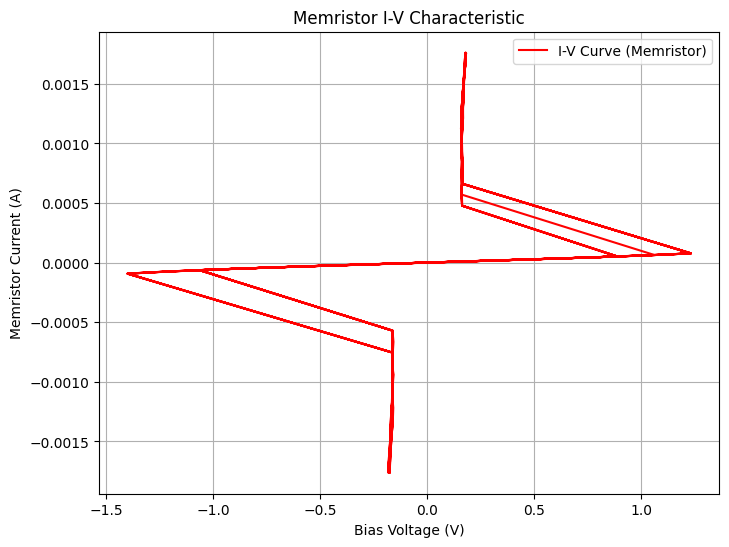
\includegraphics[width=\linewidth]{task2_memristor_iv.png}
            \caption{Measured I-V Characteristic}
        \end{figure}
    \end{columns}
\end{frame}

% ---------------------------------------------------------------------
% Slide 7: Result - Time Domain Analysis
% ---------------------------------------------------------------------
\begin{frame}{Result: Time-Dependent Behavior}
    \begin{figure}
        \centering
        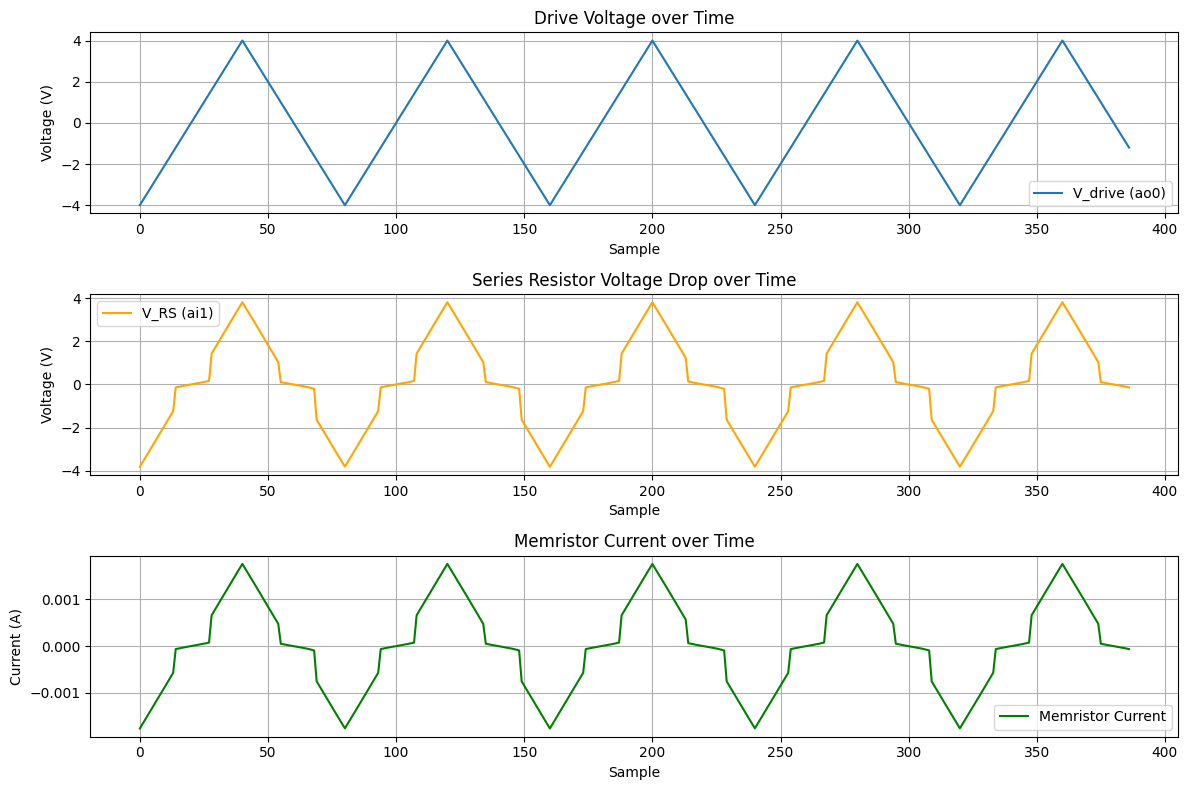
\includegraphics[width=0.6\linewidth]{task_2_three_plots.png}
        \caption{Time-dependent measurements during the I(V) sweep: (top) drive voltage, (middle) series resistor voltage drop, (bottom) calculated memristor current.}
    \end{figure}
    
    \vspace{0.4cm}
    \textbf{Observation}: The periodic current spikes (bottom graph) match the switching events in the I-V loop exactly, confirming the volatile nature of the transition is physically robust and repeatable.
\end{frame}

% ---------------------------------------------------------------------
% Slide 8: Result - Thermal Properties (Task 3a)
% ---------------------------------------------------------------------
\begin{frame}{Result: Thermal Phase Transition (Task 3)}
    \begin{columns}
        \column{0.5\textwidth}
        \begin{figure}
            \centering
            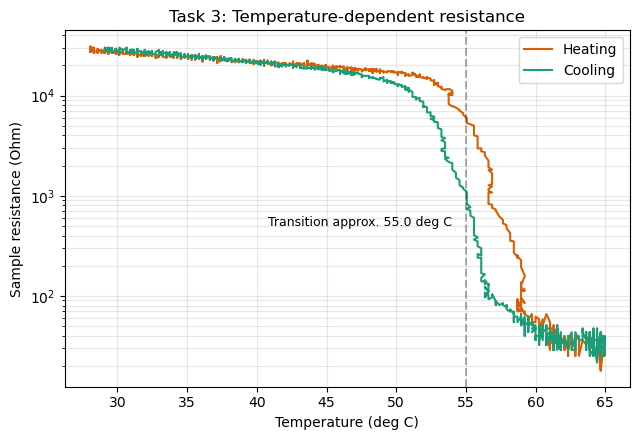
\includegraphics[width=\linewidth]{task3_rt.png}
            \caption{Resistance vs. Temperature}
        \end{figure}
        
        \column{0.5\textwidth}
        \textbf{Physical Verification} \\
        \vspace{0.3cm}
        To verify the switching mechanism, we heated the sample externally:
        \vspace{0.3cm}
        
        \textbf{Sharp Transition}: Near $57^\circ C$, resistance drops by orders of magnitude. 
        \vspace{0.3cm}
        
        This confirms that the switching observed in the I-V curves is indeed driven by the Insulator-Metal Transition phase change, rather than purely electronic breakdown effects.
    \end{columns}
\end{frame}

% ---------------------------------------------------------------------
% Slide 9: Result - Arrhenius Fitting (Task 3b)
% ---------------------------------------------------------------------
\begin{frame}{Result: Activation Energy Analysis}
    \begin{columns}
        \column{0.55\textwidth}
        \textbf{Arrhenius Analysis} \\
        \vspace{0.2cm}
        By plotting $\ln(R)$ against $1/T$, we analyzed the conduction mechanism in the insulating state.
        
        \vspace{0.6cm}
        
        \textbf{Semiconductor Behavior} \\
        The linear region indicates standard thermally activated transport ($R \propto e^{E_a/k_B T}$).
        
        \vspace{0.2cm}
        The results are consistent with standard semiconductor physics for VO2 (typically $E_a \approx 0.3-0.5 eV$), confirming the semiconducting nature of the Off state.

        \column{0.45\textwidth}
        \begin{figure}
            \centering
            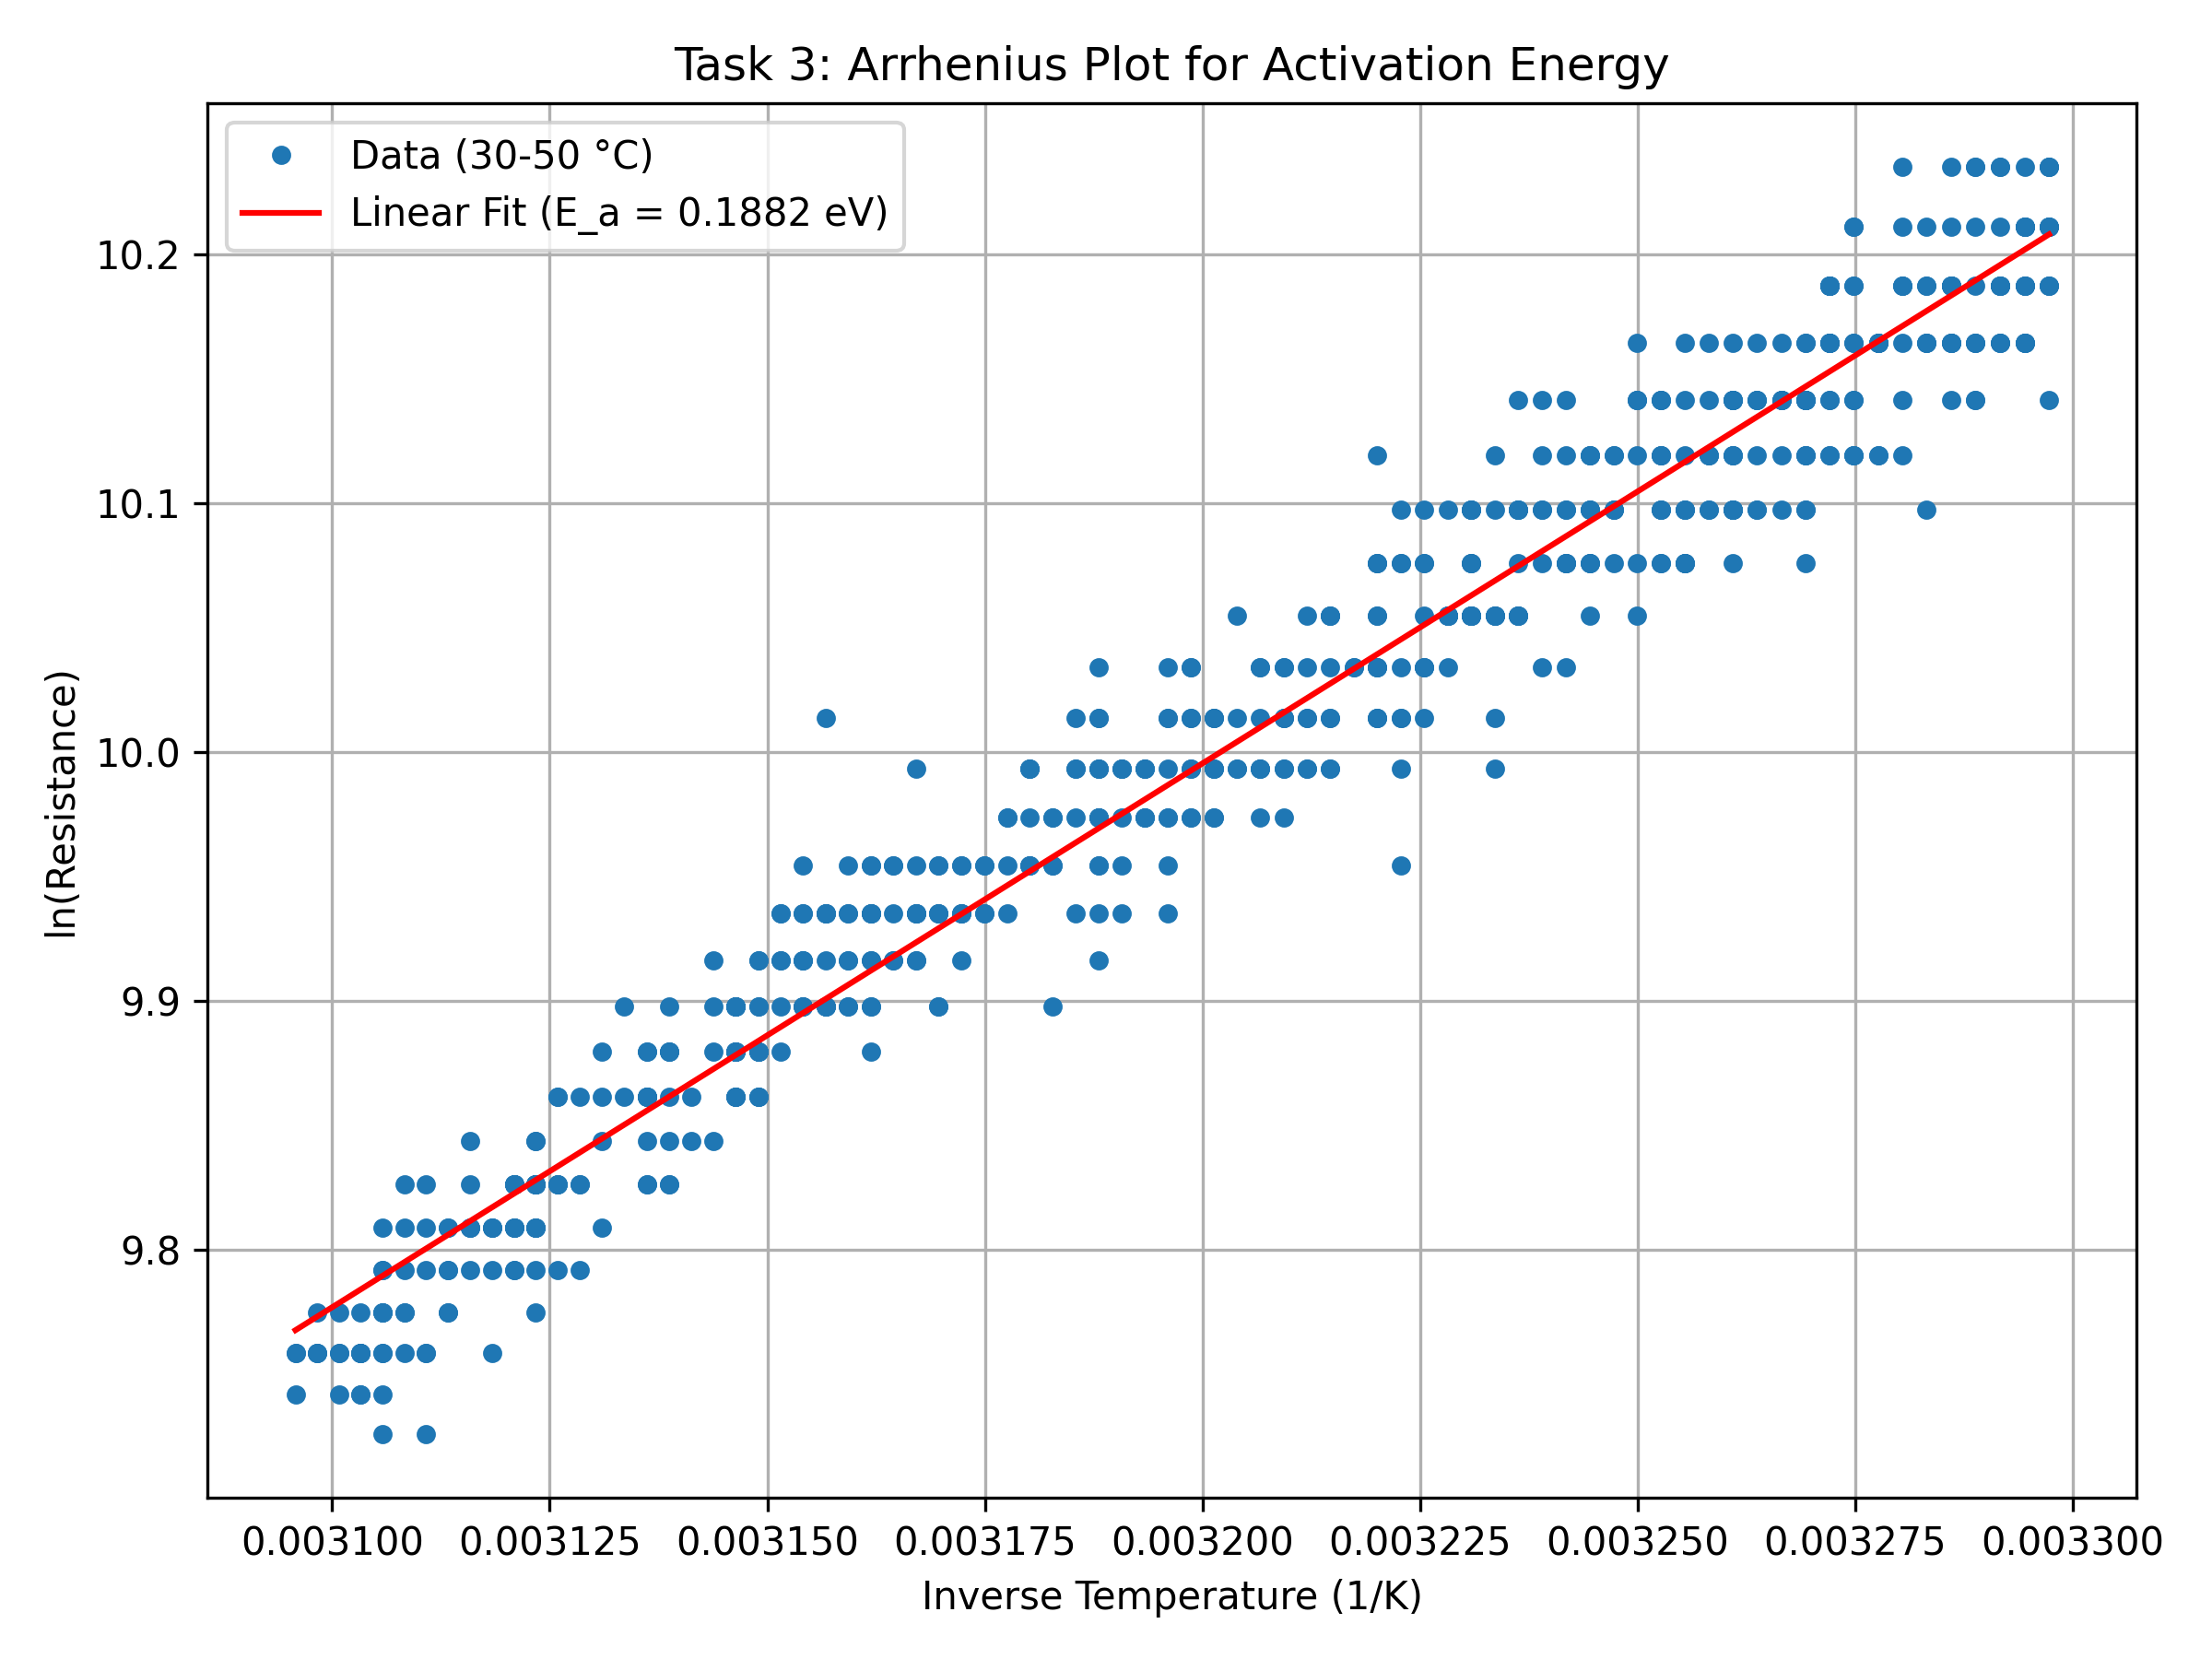
\includegraphics[width=\linewidth]{task3_arrhenius_fit.png}
            \caption{Arrhenius Fit of Resistance Data}
        \end{figure}
    \end{columns}
\end{frame}

% ---------------------------------------------------------------------
% Slide 10: Pulse Response & Dynamics (Task 4)
% ---------------------------------------------------------------------
\begin{frame}{Result: Relaxation Dynamics (Task 4)}
    \textbf{Oscillator Attempt} \\
    We aimed to construct a Pearson-Anson relaxation oscillator (Neuristor) by biasing the device in its negative differential resistance region using a capacitor.

    \vspace{0.4cm}

    \begin{columns}
        \column{0.5\textwidth}
        \textbf{Observations vs. Challenges} \\
        \vspace{0.2cm}
        We successfully triggered a single switching event, observing the characteristic current spike (shown right).
        
        \vspace{0.2cm}
        However, sustaining a stable oscillation train proved difficult. The device exhibited instability and degradation after repeated high-speed cycling. This highlights a key challenge in the field: ensuring device endurance for continuous neuromorphic operation.
        
        \column{0.5\textwidth}
        \begin{figure}
            \centering
            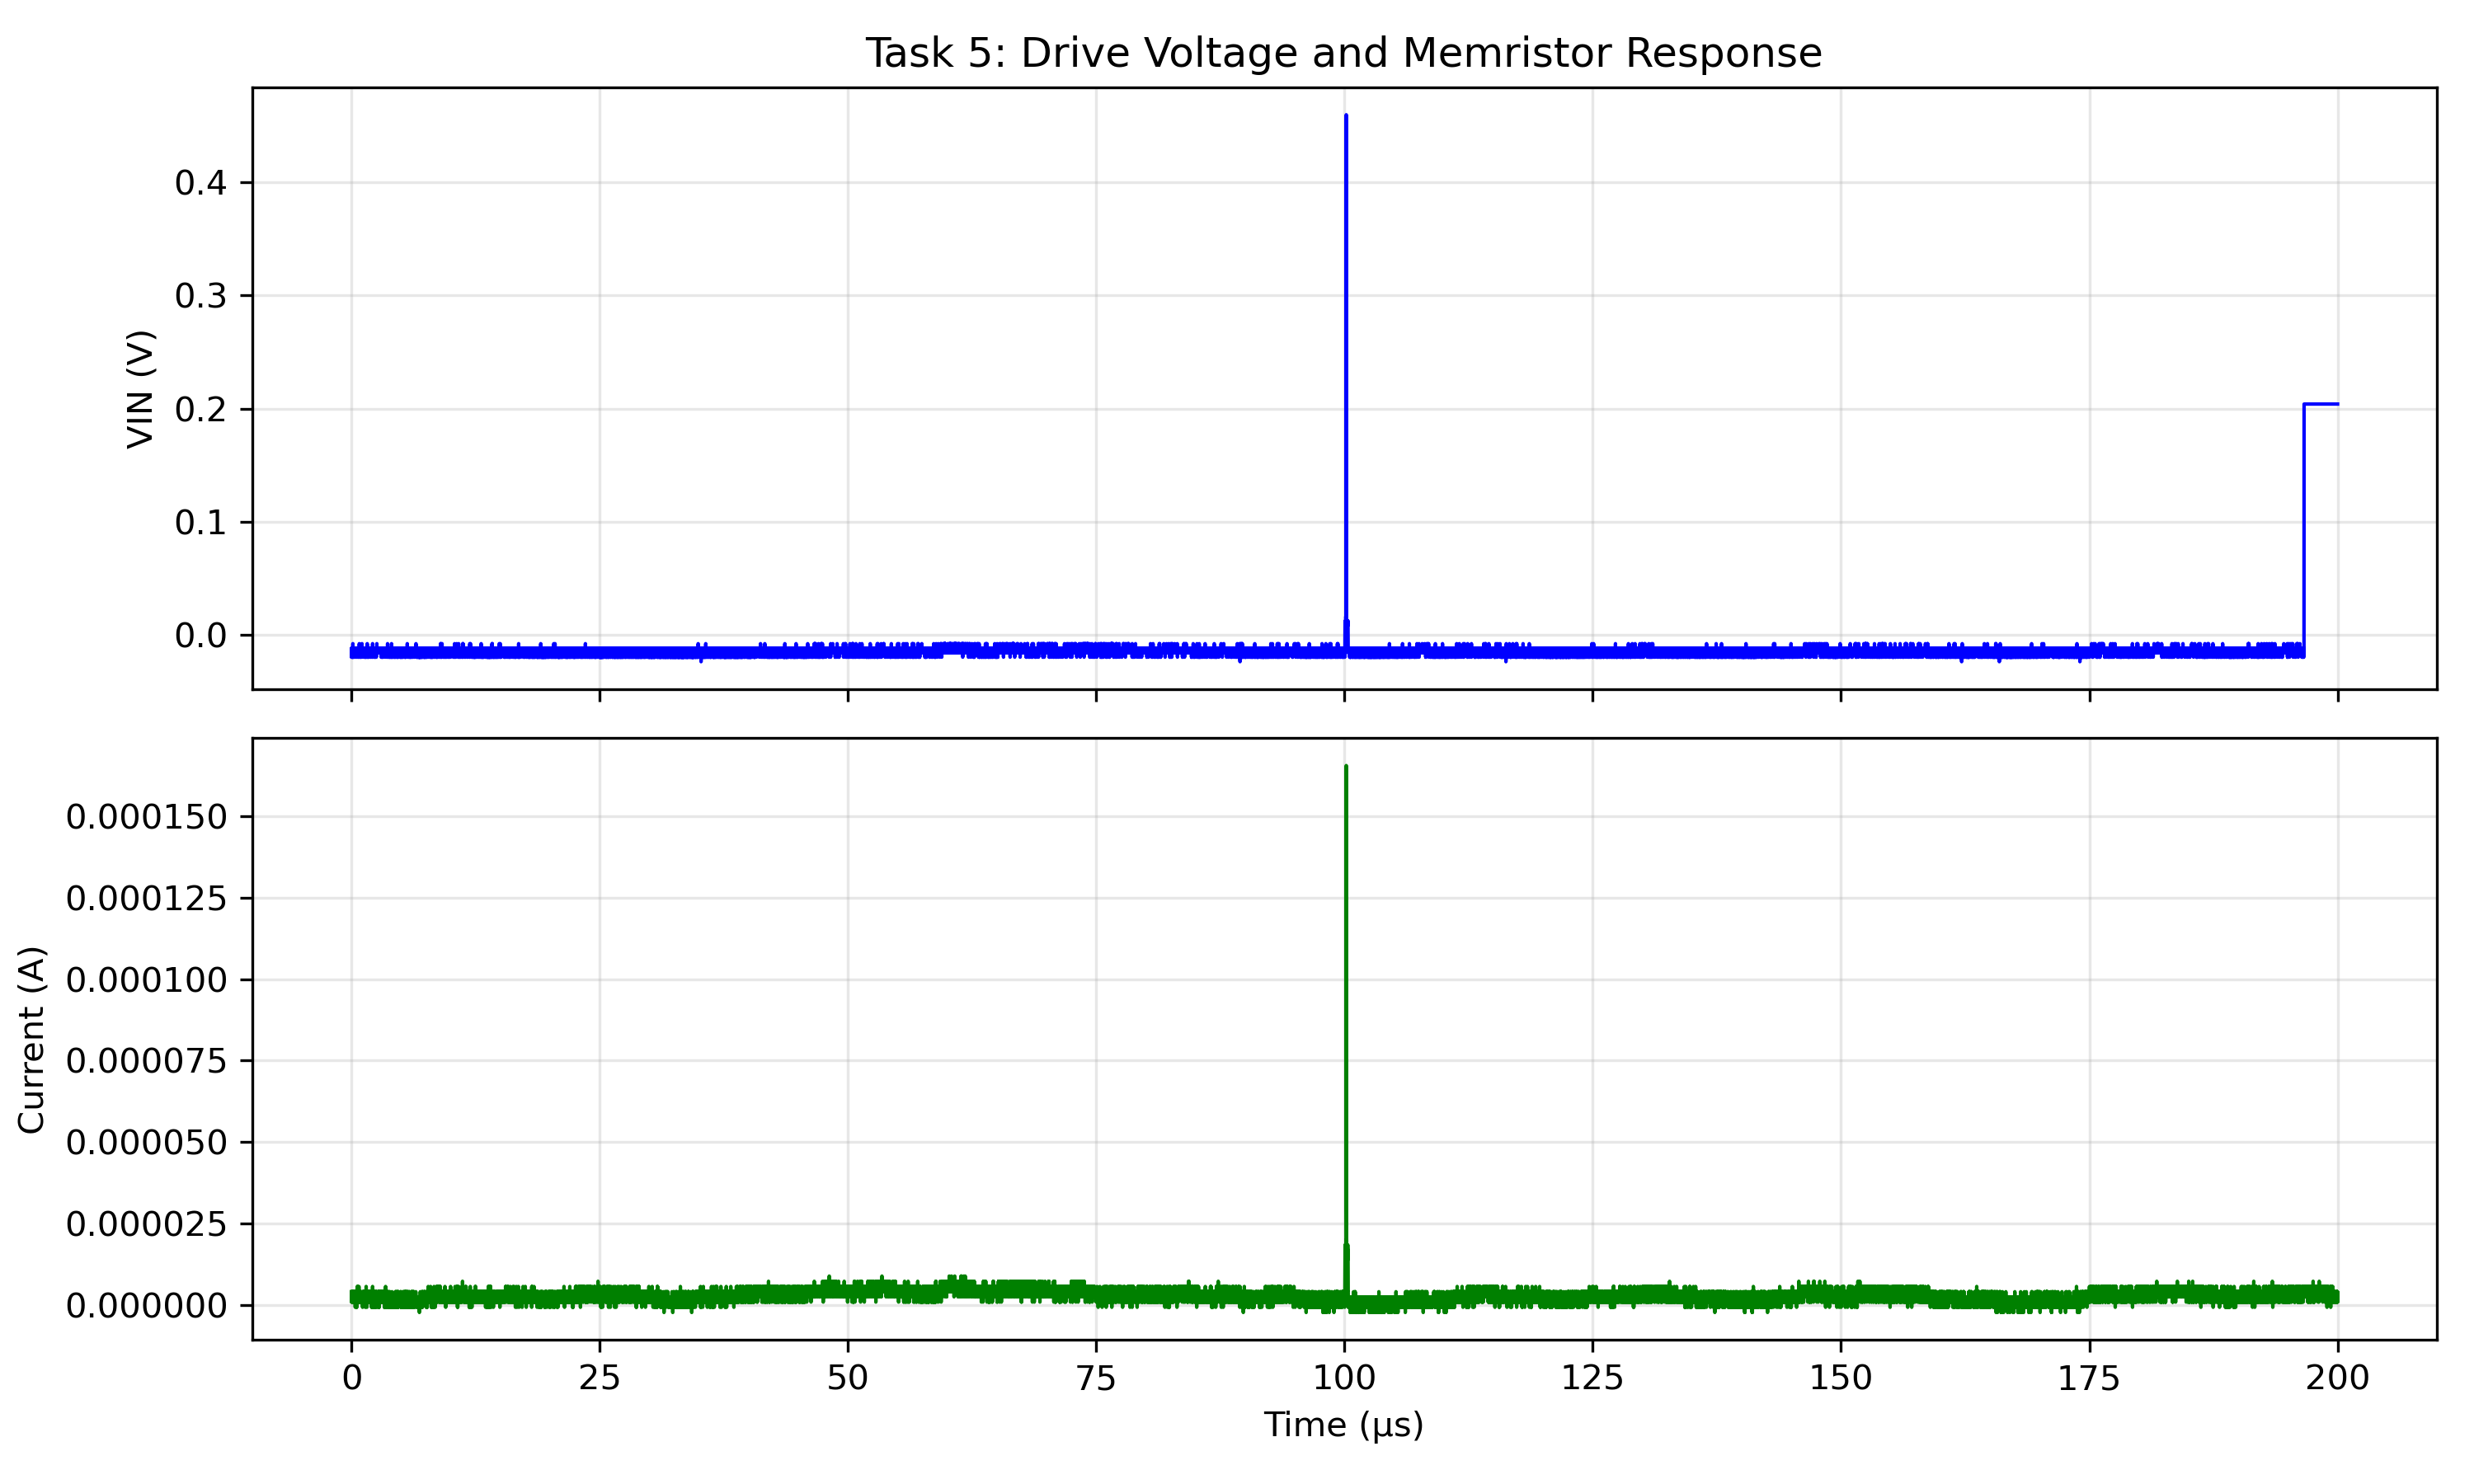
\includegraphics[width=\textwidth]{task5_full_trace.png}
            \caption{Transient Response to Pulse}
        \end{figure}
    \end{columns}
\end{frame}

% ---------------------------------------------------------------------
% Slide 11: Broad Context 1
% ---------------------------------------------------------------------
\begin{frame}{From Lab to State of the Art: Ising Machines}
    \textbf{Connecting Our Measurements to Frontier Research}
    
    \vspace{0.4cm}

    Our single-device oscillator (Right: Task 4 result) represents the fundamental building block. While maintaining stability for one device was challenging, recent breakthroughs have scaled this concept massively.
    
    \vspace{0.4cm}
    
    \textbf{The VO2 Ising Machine} \\
    Maher et al. (2024) recently demonstrated a system of \textbf{coupled VO2 oscillators} integrated on a CMOS platform \cite{maher}.
    \begin{itemize}
        \item By coupling many oscillators (like the one we measured), they created an \textbf{Ising Machine Solver}.
        \item This analog computer naturally solves NP-hard optimization problems (e.g., Graph Coloring) by letting the coupled oscillators settle into a minimum energy state (synchronization).
    \end{itemize}
\end{frame}

% ---------------------------------------------------------------------
% Slide 12: Broad Context 2
% ---------------------------------------------------------------------
\begin{frame}{From Lab to State of the Art: Biological Plausibility}
    \textbf{Stochasticity and Neural Dynamics}
    
    \vspace{0.4cm}

    In Task 3, we confirmed the thermal origin of the transition. Interestingly, the intrinsic noise and variability we observed are not just "errors"—they are features.
    
    \vspace{0.4cm}
    
    \textbf{Stochastic Neurons} \\
    Yi et al. (2018) showed that the intrinsic stochasticity in VO2 memristors closely mimics the noise found in biological ion channels \cite{yi}.
    \begin{itemize}
        \item This "noise" allows artificial neural networks to escape local minima during learning.
        \item Our verification of the switching physics confirms that these devices are not just digital switches, but biologically plausible, dynamical systems suitable for next-gen probabilistic computing.
    \end{itemize}
\end{frame}

% ---------------------------------------------------------------------
% Slide 13: Conclusion
% ---------------------------------------------------------------------
\begin{frame}{Conclusion}
    \textbf{Summary} \\
    \vspace{0.2cm}
    We successfully characterized the VO2 memristor, confirming its potential as a physical building block for neuromorphic hardware.
    
    \vspace{0.4cm}
    \textbf{Key Findings}:
    \vspace{0.2cm}
    \begin{itemize}
        \item \textbf{Robust Switching}: Demonstrated a volatile On/Off ratio $>1000$.
        \item \textbf{Physical Verification}: Confirmed the thermal origin (IMT) and activation energy.
    \end{itemize}
    
    \vspace{0.6cm}

    \textbf{Outlook} \\
    \vspace{0.2cm}
    While the switching physics is sound, improving device durability is the critical next step. Solving this will enable large-scale \textit{Oscillatory Neural Networks} capable of solving complex NP-hard problems using coupled physics \cite{maher}.
\end{frame}



% ---------------------------------------------------------------------
% Slide 13a: Acknowledgments
% ---------------------------------------------------------------------
\begin{frame}{Acknowledgments}
    \centering
    \large
    \textbf{Special Thanks to:}
    
    \vspace{1cm}
    
    \textbf{Neuromorphic Electronics Lab Staff} \\
    \textit{for guidance and supervision}
    
    \vspace{0.5cm}
    
    \textbf{Budapest University of Technology and Economics} \\
    \textit{Department of Physics}
    
    \vspace{0.5cm}
    
    \textbf{Lab Partners} \\
    \textit{Grego \& Peti}
\end{frame}

% ---------------------------------------------------------------------
% Slide 14: References
% ---------------------------------------------------------------------
\begin{frame}{References}
    \footnotesize
    \bibliographystyle{unsrt}
    \begin{thebibliography}{9}
        \bibitem{labmanual}
        Zsigmond Pollner, András Halbritter, Tímea Török et al.,
        \textit{Neuromorphic Electronics Lab Description},
        Budapest University of Technology and Economics, 2025.

        \bibitem{huang}
        Y. Huang et al.,
        ``Memristor-based hardware accelerators for artificial intelligence'',
        \textit{Nature Reviews Electrical Engineering}, 1, 286 (2024).

        \bibitem{aguirre}
        F. Aguirre et al.,
        ``Hardware implementation of memristor-based artificial neural networks'',
        \textit{Nature Communications}, 15, 1974 (2024).

        \bibitem{liu}
        H. Liu et al.,
        ``Artificial Neuronal Devices Based on Emerging Materials'',
        \textit{Advanced Materials}, 35, 2205047 (2023).

        \bibitem{maher}
        O. Maher et al.,
        ``A CMOS-compatible oscillation-based VO2 Ising machine solver'',
        \textit{Nature Communications}, 15, 3334 (2024).
        
        \bibitem{yi}
        W. Yi et al.,
        ``Biological plausibility and stochasticity in scalable VO2 active memristor neurons'',
        \textit{Nature Communications}, 9, 4661 (2018).
    \end{thebibliography}
\end{frame}

\end{document}
